\newpage
\section{Auswertung}
\subsection{Emissionsspektrum Kupfer-Röntgenröhre}
Für das Spektrum der Kupfer-Röntgenröhre ergibt sich, das gemessenen
Intensitätsmaximum bei $I_{\text{max}}=218\;$Imp/s, dafür ergibt sich
der zugehörige Braggwinkel $\Theta_{\text{max}}$ und die Wellenlänge $\lambda_{\text{max}}$
\begin{align*}
    \Theta_{\text{max}}=28.2° && \lambda_{\text{max}}=190.3\si{pm}&&E_{\text{max}}=6.52\si{keV}
\end{align*}
\begin{figure}[H]
    \centering
    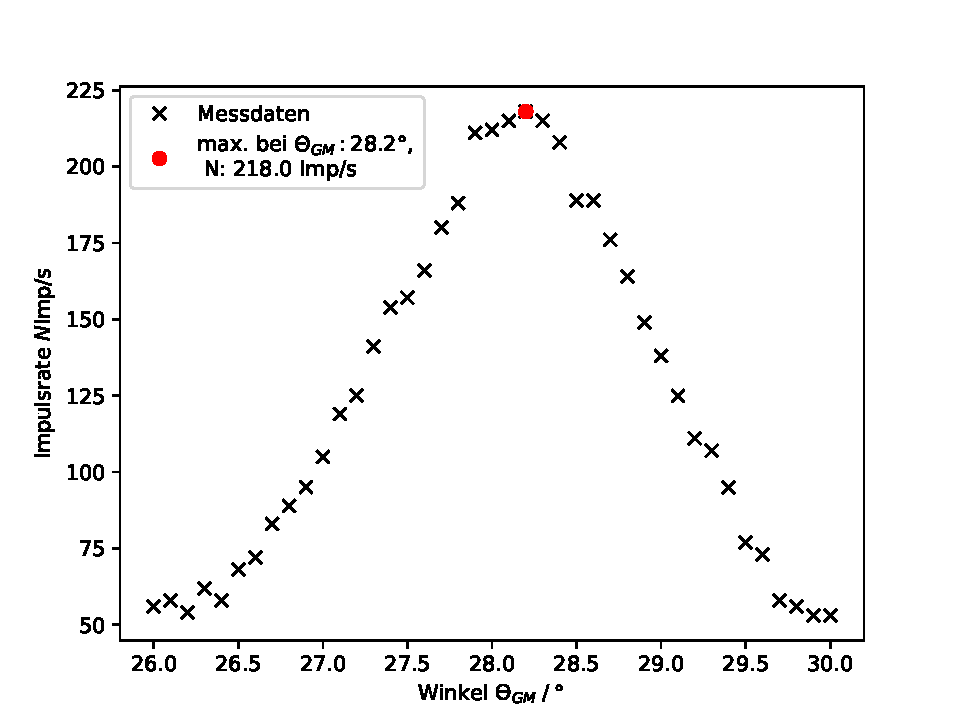
\includegraphics[width=0.7\textwidth]{plots/messdaten1.pdf}
    \caption{Die Intensitätsratenverteilung bei einem festen Kristallwinkel
    von $\Theta=14$° und mit varrierenden Geiger-Müller-Winkel $\Theta_{\text{GM}}$ mit makierten Maximum.}
\end{figure}
Für das Emissionspektrum der Kupfer-Röntgenröhre ergibt sich
\begin{figure}[H]
    \centering
    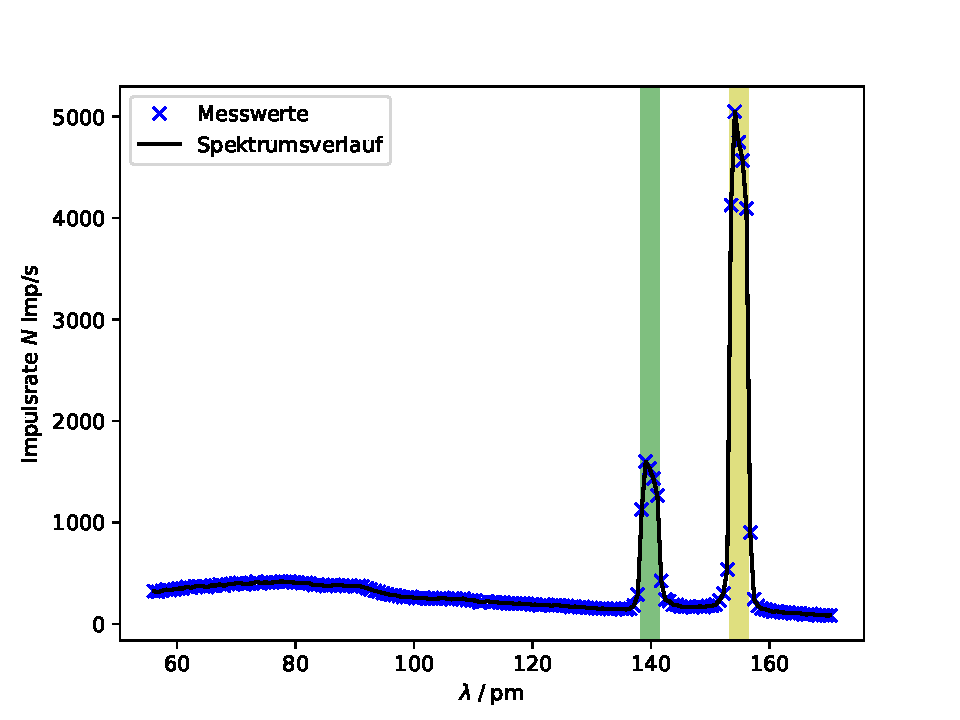
\includegraphics[width=0.7\textwidth]{plots/spektrum.pdf}
    \caption{Das Spektrum der Kupferanode. Dabei ist der erste Peak (in grün)
    die $K_{\beta}$ und der zweite Peak (in gelb) die $K_{\alpha}$ 
    Linie.}
\end{figure}
mit den Halbwertsbreiten an den Energien $E_K$ und dessen Halbwertsenenergien $\Delta E_{FWHM}$

Damit ergibt sich das Auflösungsvermögen $A$ über
\begin{equation}
    A=\frac{E_K}{\Delta E_{FWHM}}.
\end{equation}
\begin{table}[H]
    \centering
    \begin{tabular}{c | c c c c}
        \toprule
        & $E_K\;/\;\si{keV}$ & HB$\;/\;$pm & HE $\Delta E_{FMWH}\;/\;$eV&$A$\\
        \midrule
        $K_{\alpha}$ & 8.05 & 14.99 & 165.76 &48.56\\
        $K_{\beta}$  & 8.92 & 3.24  & 205.74 &43.36\\
        \bottomrule
    \end{tabular}
    \caption{Darstellung der Energien am Peak $E_K$ mit den zugehörigen Halbwertsbreiten
    HB, den Halbwertsenergien HE und dem Auflösungsverfögen $A$}
    \label{tab:tabelle1}
\end{table}
\subsection{Abschirmzahl}
Die Abschirmkonstanten $\sigma$ ergeben sich über Gl. \ref{eqn:sigma} mit $E_{\text{abs}}=8980\si{eV}$
und $E_{\alpha}$ und $E_{\beta}$ aus Tabelle \ref{tab:tabelle1} zu
\begin{align*}
    \sigma_1=&3.32,\\
    \sigma_2=&12.47,\\
    \sigma_3=&22.7.\\
\end{align*}
\subsection{Absorber}
Nun werden die Absorber mit dem MAterial Brom, Zink, Rubidium, Gallium, Rubidium und Strontium
zwischen den LiF-Kristall und den Geiger-Müller-Zähler gestellt.
Die Materiale haben folgende Kenngrößen
\begin{table}
    \centering
    \begin{tabular}{c | c c c c}
        \toprule
        &$Z$ & $E_K^{Lit}\;/\;$keV & $\Theta_K^{Lit}\;/\;$° & $\sigma_K$\\
        \midrule
        Zn & 30 & 9.65 & 18.6 & 3.56\\
        Ga & 31 & 10.37 & 17.27 &3.62\\
        Br & 35 & 13.47 & 13.20 &3.85\\
        Rb & 37 & 15.20 & 11.70 &3.95\\
        Sr & 38 & 16.10 & 11.00 &4.01\\
        Zr & 40 & 17.99 & 9.6 & 4.11\\
        \bottomrule
    \end{tabular}
    \caption{Kenngrößen zu den verschiedenen Absorbermaterialien.\cite{ref}\\
    $Z$: Ordnungszahl\\
    $E_K^{Lit}$: Literaturwert der K-Kante\\
    $\Theta_K^{Lit}$: Braggwinkel zu $E_K^{Lit}$\\
    $\sigma_K$: Abschirmkonstante}
    \label{tab:kenngroesse}
\end{table}
\subsubsection{Brom}
Über das Intensitätsmaximum $I_K^{max}$ und das Intensitätsminimum $I_K^{min}$
wird mit
\begin{equation}
    I_K=I_K^{min}+\frac{I_K^{max}-I_K^{min}}{2}
    \label{eqn:intensität}
\end{equation}
die Mitte der K-Kante gewählt. Über den zugehörigen Winke $\Theta$ kann nun mit
Gl. \ref{eqn:bragg} die Absibrtionenergie $E_{K,abs}$ der K-Kante ermittelt werden.
Weitergehen folgt nach Gl. \ref{eqn:sigmaZ} die Abschirmkonstante $\sigma_K$.\\
Es ergibt sich:
\begin{table}
    \centering
    \begin{tabular}{c | c c c c c c}
        \toprule
        &$\Theta\;/\;$° & $E_{K,abs}\,/\;$keV & $I_K^{min}\;/\;\frac{Imp}{s}$ & $I_K^{max}\;/\;\frac{Imp}{s}$ & $I_K\;/\;\frac{Imp}{s}$ & $\sigma_K$\\
        \midrule
        Brom & 13.2 & 13.49 & 9.0 & 27.0 & 18.0 & 3.84\\
        Zink & 18.7 & 9.61 & 55.0 & 102.0 & 78.5 & 3.64\\
        Gallium & 17.375 & 10.34 & 66.0 & 121.0 & 93.5 & 3.70\\
        Rubidium & 11.8 & 15.06 & 12.0 & 64.0 & 38.0 & 4.11\\
        Strontium & 11.1 & 16.00 & 50.0 & 193.0 & 121.5 & 4.12\\
        Zirkonium & 9.95 & 17.83 & 112.0 & 282.0 & 197.0 & 4.28\\
        \bottomrule
    \end{tabular}
    \caption{Die Lage der Absorbtionskante und Absorbtionsenergie $E_{K,abs}$ von Brom.
        Sowie die zugehörigen Intensitäten $I_K^{min}$,$I_K^{max}$,$I_K$ und die Abschirmkonstante $\sigma$.}
\end{table}


\label{sec:Auswertung}
